% Intended LaTeX compiler: pdflatex
\documentclass[11pt]{article}
\usepackage[utf8]{inputenc}
\usepackage[T1]{fontenc}
\usepackage{graphicx}
\usepackage{longtable}
\usepackage{wrapfig}
\usepackage{rotating}
\usepackage[normalem]{ulem}
\usepackage{amsmath}
\usepackage{amssymb}
\usepackage{capt-of}
\usepackage{hyperref}
\author{Construção de compiladores I}
\date{}
\title{Expressões regulares}
\hypersetup{
 pdfauthor={Construção de compiladores I},
 pdftitle={Expressões regulares},
 pdfkeywords={},
 pdfsubject={},
 pdfcreator={Emacs 28.2 (Org mode 9.7)}, 
 pdflang={English}}
\begin{document}

\maketitle
\section*{Objetivos}
\label{sec:org328c7e8}

\subsection*{Objetivos}
\label{sec:org63cd279}

\begin{itemize}
\item Apresentar como utilizar expressões regulares para
especificar a estrutura léxica de linguagens.
\end{itemize}
\subsection*{Objetivos}
\label{sec:orgf654ed2}

\begin{itemize}
\item Mostrar como produzir autômatos não determinísticos a partir de expressões regulares.

\item Mostrar como obter um autômato determinístico a partir de um não determinístico.
\end{itemize}
\section*{Expressões regulares}
\label{sec:org7c6a125}

\subsection*{Expressões regulares}
\label{sec:org732cf12}

\begin{itemize}
\item Forma algébrica para especificar linguagens regulares.

\item Linguagens regulares: aceitas por AFDs
\end{itemize}
\subsection*{Expressões regulares}
\label{sec:orgcce89b5}

\begin{itemize}
\item Sintaxe
\end{itemize}

\begin{array}{lcl}
e & \to  & \emptyset\:\mid\:\lambda\:\mid\: a\:\mid\:e\,e\:\mid\:e\,+\,e\:\mid\:e^*\\
\end{array}
\subsection*{Expressões regulares}
\label{sec:org0335f10}

\begin{itemize}
\item Expressões regulares denotam \textbf{linguagens}.
\end{itemize}
\subsection*{Expressões regulares}
\label{sec:org57e1ec4}

\begin{itemize}
\item Semântica:
\end{itemize}

\begin{array}{lcl}
\lbrack\!\lbrack \emptyset \rbrack\!\rbrack    & =  & \emptyset\\
\lbrack\!\lbrack \lambda \rbrack\!\rbrack      & =  & \{\lambda\}\\
\lbrack\!\lbrack a \rbrack\!\rbrack            & =  & \{a\}\\
\lbrack\!\lbrack e_1\!e_2 \rbrack\!\rbrack     & =  & \lbrack\!\lbrack e_1\rbrack\!\rbrack\:\lbrack\!\lbrack e_2\rbrack\!\rbrack\\
\lbrack\!\lbrack e_1\!+\!e_2 \rbrack\!\rbrack  & =  & \lbrack\!\lbrack e_1\rbrack\!\rbrack\!\cup\!\lbrack\!\lbrack e_2\rbrack\!\rbrack\\
\lbrack\!\lbrack e_1^*\rbrack\!\rbrack  & =  & \lbrack\!\lbrack e_1\rbrack\!\rbrack^*\\
\end{array}
\subsection*{Expressões regulares}
\label{sec:orgf4d9fd9}

\begin{itemize}
\item Expressões regulares são equivalentes a \textbf{autômatos finitos não determinísticos}.

\item Equivalência definida pela \textbf{construção de Thompson}.
\end{itemize}
\section*{Autômatos não determinísticos}
\label{sec:org0b2ab18}

\subsection*{Autômatos não determinísticos}
\label{sec:org188a81f}

\begin{itemize}
\item Um AFN \(M=(E,\Sigma,\delta,I,F)\):
\begin{itemize}
\item \(E\) : conjunto de estados
\item \(\Sigma\): alfabeto
\item \(\delta : E\times\Sigma\to\mathcal{P}(E)\): função de transição.
\item \(I \subseteq E\): conjunto de estados iniciais.
\item \(F\subseteq E\): conjunto de estados finais.
\end{itemize}
\end{itemize}
\subsection*{Autômatos não determinísticos}
\label{sec:org70d41af}

\begin{itemize}
\item Exemplo: \((0+1)^*00\)
\end{itemize}

\begin{center}
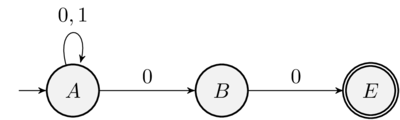
\includegraphics[width=.9\linewidth]{./imgs/image7.png}
\end{center}
\subsection*{Autômatos não determinísticos.}
\label{sec:org8c7307c}

\begin{itemize}
\item Seja \(M=(E,\Sigma,\delta,I,F)\) um AFN.

\item O AFD equivalente é \((\mathcal{P}(E),\Sigma,\delta',I, F')\):
\begin{itemize}
\item \(\delta'(X,a) = \bigcup_{e\in X}\delta(e,a)\).
\item \(F' = \{X\,|\, X \cap F = \emptyset\}\).
\end{itemize}
\end{itemize}
\subsection*{Autômatos não determinísticos}
\label{sec:org9974da8}

\begin{itemize}
\item Implementação em Haskell
\end{itemize}

\begin{verbatim}
data NFA a
  = NFA {
      numberOfStates :: Int
    , nfaStart :: Set a
    , nfaDelta :: a -> Char -> Set a
    , nfaFinals :: Set a
    }
\end{verbatim}
\subsection*{Autômato não determinísticos}
\label{sec:org5292a16}

\begin{itemize}
\item Implementação em Haskell
\end{itemize}

\begin{verbatim}
subset :: Ord a => NFA a -> DFA (Set a)
subset m
  = DFA {
      start  = nfaStart m
    , delta  = \ es c ->
        Set.unions (map (flip (nfaDelta m) c) (Set.elems es))
    , finals = \ es -> not (disjoint es (nfaFinals m))
    }
\end{verbatim}
\section*{Construção de Thompson}
\label{sec:org8d48d12}

\subsection*{Construção de Thompson}
\label{sec:org95731ba}

\begin{itemize}
\item Mostra como obter um AFN a partir de uma expressão regular.

\item Estratégia utilizada por ferramentas de geração de analisadores léxicos.
\end{itemize}
\subsection*{Construção de Thompson}
\label{sec:org5fd2983}

\begin{itemize}
\item AFN para \(e = \emptyset\).
\end{itemize}

\begin{center}
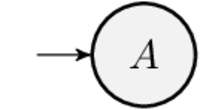
\includegraphics[width=.9\linewidth]{./imgs/image1.png}
\end{center}
\subsection*{Construção de Thompson}
\label{sec:orga125bd8}

\begin{itemize}
\item AFN para \(e = \lambda\).
\end{itemize}

\begin{center}

\includegraphics[width=.9\linewidth]{./imgs/image2.png}
\end{center}
\subsection*{Construção de Thompson}
\label{sec:orge0cc7b8}

\begin{itemize}
\item AFN para \(e = a\).
\end{itemize}

\begin{center}
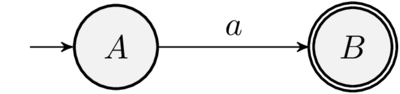
\includegraphics[width=.9\linewidth]{./imgs/image3.png}
\end{center}
\subsection*{Construção de Thompson}
\label{sec:orgb545ffd}

\begin{itemize}
\item AFN para \(e = e_1 + e_2\).
\end{itemize}

\begin{center}
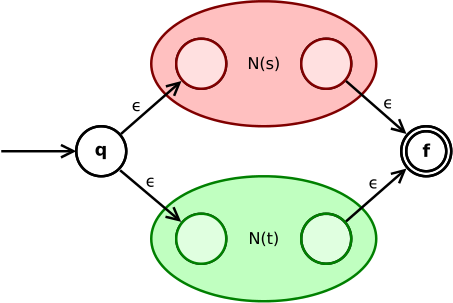
\includegraphics[width=.9\linewidth]{./imgs/image4.png}
\end{center}
\subsection*{Construção de Thompson}
\label{sec:orgb98a6a0}

\begin{itemize}
\item AFN para \(e = e_1\:e_2\).
\end{itemize}

\begin{center}
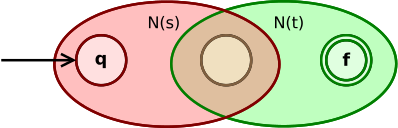
\includegraphics[width=.9\linewidth]{./imgs/image5.png}
\end{center}
\subsection*{Construção de Thompson}
\label{sec:org4365e41}

\begin{itemize}
\item AFN para \(e = e_1^*\).
\end{itemize}

\begin{center}
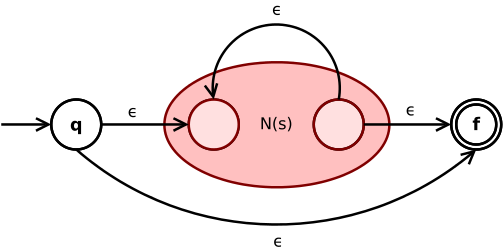
\includegraphics[width=.9\linewidth]{./imgs/image6.png}
\end{center}
\subsection*{Construção de Thompson}
\label{sec:org3bed592}

\begin{itemize}
\item Como implementar?
\begin{itemize}
\item AFNs para casos bases.
\item Funções para combinar AFNs.
\end{itemize}
\end{itemize}
\subsection*{Construção de Thompson}
\label{sec:org937f273}

\begin{itemize}
\item AFN para \(\emptyset\).
\end{itemize}

\begin{verbatim}
emptyNFA :: NFA Int
emptyNFA
  = NFA 0 Set.empty
          (\ _ _ -> Set.empty)
          Set.empty
\end{verbatim}
\subsection*{Construção de Thompson}
\label{sec:org261e17e}

\begin{itemize}
\item AFN para \(\{\lambda\}\).
\end{itemize}

\begin{verbatim}
lambdaNFA :: NFA Int
lambdaNFA
  = NFA 1 one
          (\ _ _ -> Set.empty)
          one
    where
      one = Set.singleton 1
\end{verbatim}
\subsection*{Construção de Thompson}
\label{sec:org19f06e9}

\begin{itemize}
\item AFN para \(\{a\}\).
\end{itemize}

\begin{verbatim}
chrNFA :: Char -> NFA Int
chrNFA c
  = NFA 2 zero f one
    where
      zero = Set.singleton 0
      one = Set.singleton 1
      err = Set.singleton 2
      f 0 x = if c == x then one
              else err
      f _ _ = err
\end{verbatim}
\subsection*{Construção de Thompson}
\label{sec:org0a27247}

\begin{itemize}
\item Antes de definir funções para combinar AFNs,
precisamos garantir que estes não possuam estados em comum.
\end{itemize}
\subsection*{Construção de Thompson}
\label{sec:org93450d5}

\begin{itemize}
\item Para isso, vamos ``renomear'' estados de um AFN.
\end{itemize}

\begin{verbatim}
shift :: Int -> Set Int -> Set Int
shift n = Set.fromAscList . map (+ n) . Set.toAscList
\end{verbatim}
\subsection*{Construção de Thompson}
\label{sec:orge0cbd3a}

\begin{itemize}
\item AFN para \(e_1 + e_2\).
\end{itemize}

\begin{verbatim}
unionNFA :: NFA Int -> NFA Int -> NFA Int
unionNFA m1 m2
  = NFA {
      numberOfStates = n1 + n2
    , nfaStart = Set.union (nfaStart m1) (shift n1 (nfaStart m2))
    , nfaDelta = f
    , nfaFinals = Set.union (nfaFinals m2) (shift n1 (nfaFinals m2))
    }
    where
      n1 = numberOfStates m1
      n2 = numberOfStates m2
      f s c = if s < n1 then nfaDelta m1 s c
              else shift n1 (nfaDelta m2 (s - n1) c)
\end{verbatim}
\subsection*{Construção de Thompson}
\label{sec:orgeeddfbe}

\begin{itemize}
\item AFN para \(e_1\:e_2\).
\end{itemize}

\begin{verbatim}
concatNFA :: NFA Int -> NFA Int -> NFA Int
concatNFA m1 m2
    = NFA {
        numberOfStates = n1 + n2
      , nfaStart = newStart
      , nfaDelta = newDelta
      , nfaFinals = newFinals
      }
      where
        n1 = numberOfStates m1
        n2 = numberOfStates m2
\end{verbatim}
\subsection*{Construção de Thompson}
\label{sec:org3ae0779}

\begin{itemize}
\item AFN para \(e_1\:e_2\) (continuação).
\end{itemize}

\begin{verbatim}
start1 = nfaStart m1
final1 = nfaFinals m1
newStart = if disjoint start1 final1
           then start1
            else Set.union start1 (shift n1 final1)
newFinals = shift n1 final1
newDelta e c = if e < n1 then
                 if disjoint (nfaDelta m1 e c) final1
                 then nfaDelta m1 e c
                 else Set.union (nfaDelta m1 e c) start1
               else shift n1 (nfaDelta m2 (e - n1) c)
\end{verbatim}
\subsection*{Construção de Thompson}
\label{sec:org9ba737e}

\begin{itemize}
\item AFN para \(e = e_1^*\).
\end{itemize}

\begin{verbatim}
starNFA :: NFA Int -> NFA Int
starNFA m1
  = NFA {
      numberOfStates = numberOfStates m1
    , nfaStart = nfaStart m1
    , nfaDelta = newDelta
    , nfaFinals = nfaStart m1
    }
    where
      newDelta e c
        = let r = nfaDelta m1 e c
          in if disjoint r (nfaFinals m1)
             then r
             else Set.union r (nfaStart m1)
\end{verbatim}
\subsection*{Construção de Thompson}
\label{sec:org232dbd1}

\begin{itemize}
\item Convertendo uma ER em um DFA:
\end{itemize}

\begin{verbatim}
toDFA :: Regex -> DFA (Set Int)
toDFA = subset . thompson
\end{verbatim}
\subsection*{Construção de Thompson}
\label{sec:orga603a9c}

\begin{itemize}
\item Construindo o AFD para um conjunto de REs.
\end{itemize}

\begin{verbatim}
lexer :: [Regex] -> DFA (Set Int)
lexer = subset . foldr unionNFA emptyNFA . map thompson
\end{verbatim}
\section*{Concluindo}
\label{sec:orge9bc5f1}

\subsection*{Concluindo}
\label{sec:orge4eb9df}

\begin{itemize}
\item Revisamos REs, AFNs e sua relação com AFDs.

\item Apresentamos como construir AFDs a partir de expressões regulares.
\end{itemize}
\subsection*{Concluindo}
\label{sec:org1da90ca}

\begin{itemize}
\item Próxima aula: Derivadas de expressões regulares e geradores de analisadores léxicos.
\end{itemize}
\section*{Exercícios}
\label{sec:org631b480}

\subsection*{Exercícios}
\label{sec:org8519d39}

\begin{itemize}
\item Construa um analisador léxico para a linguagem IMP utilizando o arcabouço baseado
em expressões regulares e AFDs.
\end{itemize}
\end{document}
